% !TEX encoding = utf8
% !TEX root = ../main.tex

\chapter{Classificazione di immagini telerilevate ad alta risoluzione} 
\label{cap:telerilevamento} 

Il telerilevamento (\emph{remote sensing}) viene definito come la disciplina che permette di ricavare informazioni su oggetti posti a distanza da uno o più sensori, che ne permettono l'estrazione. 
Questa definizione generale comprende un vasto range di sotto-discipline atte ad estrarre informazioni, tra le quali l'estrapolazione di dati di interesse ambientale, l'identificazione di oggetti posti sul fondale marino o fino a tecniche di l'\emph{human detection}.
Nel nostro caso, ci focalizzeremo in particolare nell'ambito dell'Osservazione della Terra (\emph{Earth Observation}, EO) in cui l'oggetto da analizzare sarà una porzione di suolo.
\clearpage


\section{Cenni sul Telerilevamento}


\subsection{Sensori}
Nel caso di telerilevamento al fine di \emph{EO}, i sensori sono tipicamente montati su un aereo (sensore aviotrasportato) o su un satellite (sensore satellitare), i quali trasducono l'onda elettromagnetica incidente su di essi in una immagine digitale, al fine di essere elaborata da un calcolatore. 
I sensori hanno, infatti, lo scopo di acquisire parametri ambientali utili ad una successiva elaborazione delle informazioni, seguendo il procedimento rappresentato dallo schema a blocchi riportato in Figura \ref{fig:flussosistema}.

\begin{figure}[!ht]
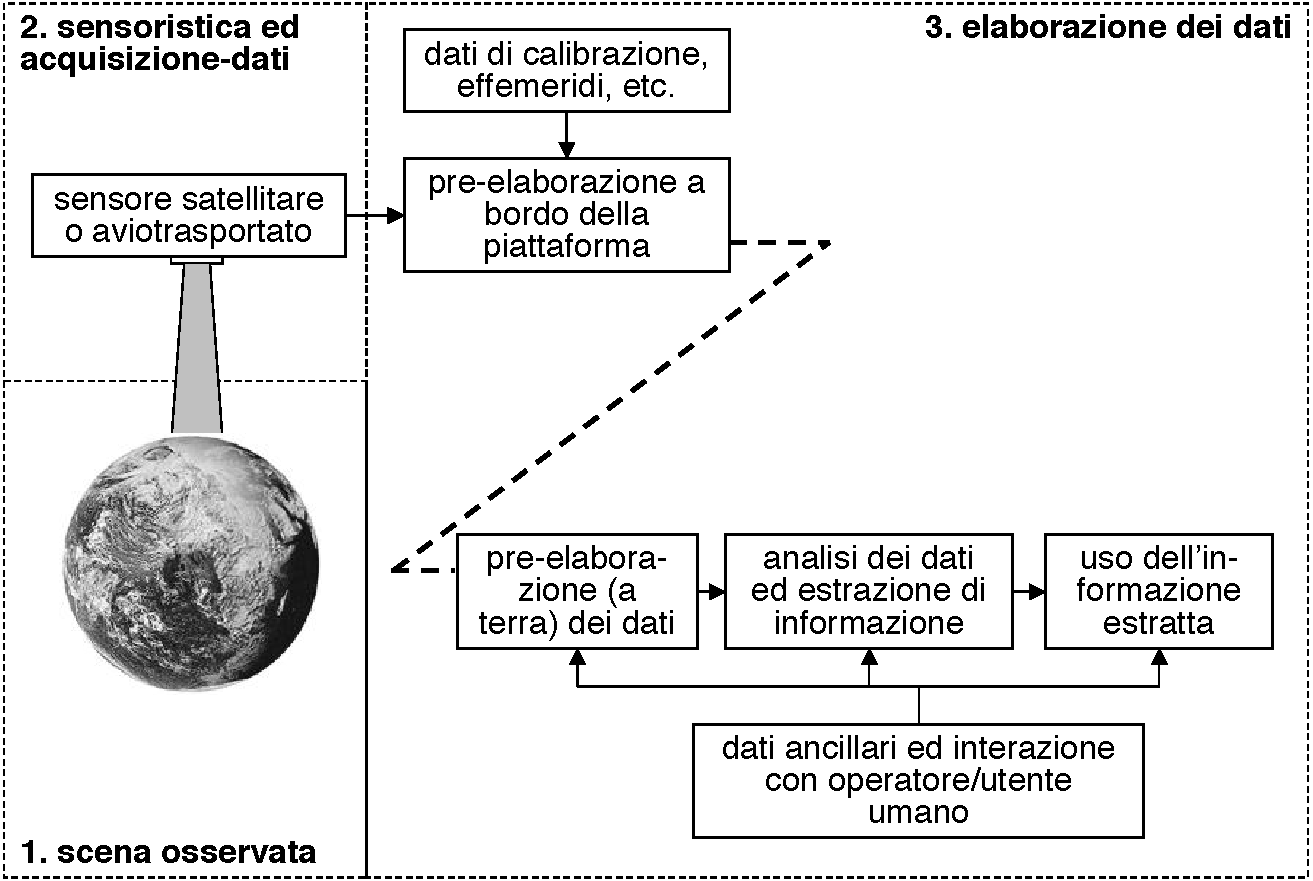
\includegraphics[width=1\textwidth]{flussosistema}
\caption{Schema a blocchi (concettuale) di un sistema di telerilevamento.}
\label{fig:flussosistema}
\end{figure}

Il procedimento è il seguente:
\begin{itemize}
\item innanzitutto la radiazione emessa dall'oggetto in esame (ad esempio una porzione di suolo) viene ricevuta in ingresso al fotorivelatore, per essere elaborata dal sistema;
\item il sistema di elaborazione prevede in taluni casi, una fase iniziale di pre-elaborazione dei dati a bordo della piattaforma, basata su informazioni inerenti ai sensori (ad esempio dati di calibrazione del sensore) o alla piattaforma stessa (ad esempio effemeridi);
\item successivamente, vengono effettuate operazioni di pre-elaborazione analoghe ma a terra, aventi fini quali un'ulteriore calibrazione dei dati o la rimozione di distorsioni geometriche o radiometriche dovute al movimento della piattaforma;
\item infine il sistema procede all'elaborazione vera e propria dei dati telerilevati al fine di estrarre l'informazione che viene infine fornita all'utilizzatore.
\end{itemize}


\subsection{Tipologie di sensori}

Generalmente, i sensori per telerilevamento vengono divisi in due macro-famiglie, i sensori passivi e quelli attivi.
La prima tipologia non trasmette alcun segnale ma, bensì, riceve unicamente la radiazione emessa dall'oggetto in esame, ovvero la radiazione elettromagnetica emessa dalla porzione di superficie, la quale può essere spontanea (tipicamente radiazione infrarossa) oppure la radiazione riflessa o diffusa proveniente dal sole (radiazione infrarossa e/o nello spettro del visibile).
I sensori attivi, invece, trasmettono un'onda elettromagnetica nella direzione della superficie in esame e analizzano il segnale (simile ad un eco sonoro) ritrasmesso dalla porzione di suolo stessa.
Tali onde elettromagnetiche sono tipicamente segnali laser, i quali usano sensori \emph{LIght Detection And Ranging} (LIDAR), oppure a microonde, analizzati tramite sensori \emph{RAdio Detection And Ranging} (RADAR).
\\

La nostra trattazione si baserà unicamente su segnali rilevati tramite sensori passivi, in particolare sensori ottici.  


\subsection{Il ruolo della risoluzione}
Un parametro di vitale importanza per un sensore orientato all' \emph{EO} è la risoluzione, con la quale si intende una risoluzione spaziale, temporale e spettrale.
La prima rappresenta il più piccolo dettaglio della superficie in esame che risulta distinguibile dopo essere stata estratta dal sensore, in particolare questo parametro viene espresso come la grandezza della superifcie rappresentata da un singolo pixel.
La risoluzione temporale, invece, è definita come la frequenza con cui il sensore osserva una stessa porzione di superifice. 
Essa è infatti definita come il tempo intercorso tra due passaggi del sensore sulla stessa area geografica, intervallo di tempo che può variare dal mese fino, addirittura, al singolo giorno.
Infine, la risoluzione spettrale viene definita come il numero di bande (o canali) misurate per ciascun pixel e dalla larghezza di banda di ogni singolo canale. Ad esempio, il sensore iperspettrale AVIRIS campiona la radiazione incidente acquisendo $224$ bande distinte, ognuna avente una larghezza pari a $9.3$ nm, rendendolo un sensore ad alta risoluzione temporale, a differenza di sensori pancromatici che elaborano solamente l'intervallo di lunghezze d'onda della radiazione visibile.


\subsection{Telerilevamento tramite sensori ottici multispettrali}
La nostra analisi si focalizzerà su sensori passivi multispettrali costituiti da sistemi di elaborazione ottica, i quali indirizzano la radiazione incidente su uno o più foto-rivelatori, che trasducono una grandezza fisica (l'intensità della radiazione elettromagnetica) in una tensione elettrica. Queste tipologie di sensori vengono trasportati da una piattaforma che viaggia ad una quota h e fa percorrere al sensore una direzione di volo (direzione \emph{in-track}), lungo la quale esso effettua uno scan lungo la direzione ortogonale (detta direzione \emph{cross-track}).
I sensori possono essere suddivisi, in base alla tecnica di scansione utilizzata, in tre famiglie:

\begin{itemize}
\item \emph{Line Scanner}, sensori che montano un solo rivelatore ottico che scandisce l'intera riga per mezzo di uno specchio oscillante;
\item \emph{Whiskbroom Scanner}, i quali possiedono un array di rivelatori orientati secondo la direzione \emph{in-track}, che scandiscono, in questo modo, più linee alla volta; 
\item \emph{Pushbroom Scanner}, contenenti un numero elevato di foto-rivelatori, lungo la direzione \emph{cross-track}, i quali permettono di scandire intere righe dell'immagine senza l'utilizzo di parti mobili.
\end{itemize}

\begin{figure}[htbp]
\centering
\subfigure[]{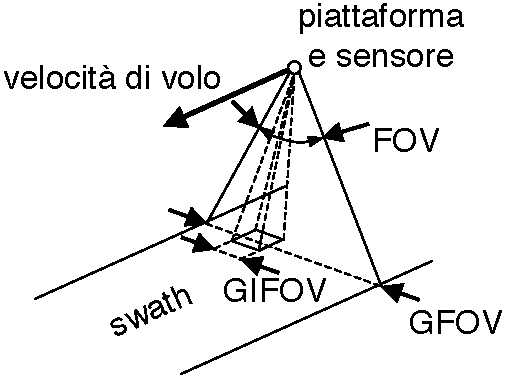
\includegraphics[width=0.3\textwidth]{linescanner}}
\qquad
\subfigure[]{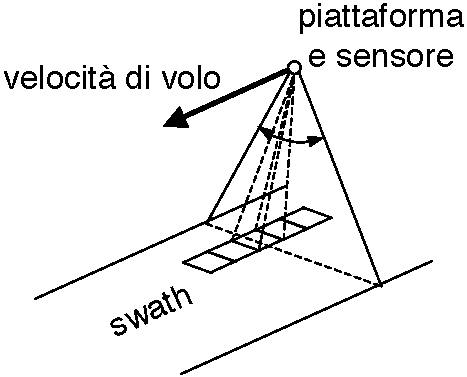
\includegraphics[width=0.3\textwidth]{whiskbroom}}
\qquad
\subfigure[]{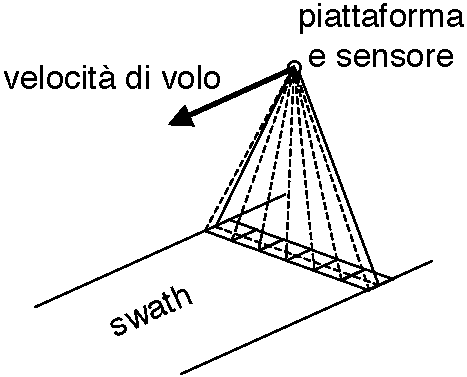
\includegraphics[width=0.3\textwidth]{pushbroom}}
\qquad
\caption{Metodi di scansione rispettivamente dei \emph{line scanner} (a), \emph{whiskbroom scanner} (b) e \emph{pushbroom scanner} (c).}
\end{figure}

Parametri chiave dei sensori ottici sono il cosiddetto \emph{Field Of View} (FOV), ovvero l'ampiezza espressa in radianti della zona di suolo osservata in direzione \emph{cross-track} e la corrispondente larghezza a terra della striscia osservata, il \emph{Ground Field Of View} (GFOV).
In modo analogo, l'estensione angolare di ogni foto-rivelatore è detta \emph{Istantaneous Field Of View} (IFOV) mentre la sua proiezione viene detta \emph{Ground Istantaneous Field Of View} (GIFOV).
Fra queste grandezze esistono delle relazioni espresse dalle seguenti equazioni:
\begin{equation}
GFOV = 2h\tan{\frac{FOV}{2}} 
\end{equation}
\begin{equation}
GIFOV = 2h\tan{\frac{IFOV}{2}}
\end{equation}
Tali sensori ottici passivi analizzano vari range di frequenze che tendenzialmente vanno dall'infrarosso termico (TIR, 8-9.5 $\si{\micro\m}$, 10-14 $\si{\micro\m}$) allo spettro del visibile (VIS, 0.4-0.7 $\si{\micro\m}$), rilevando la radianza spettrale, grandezza che permette di descrivere la distribuzione spaziale della radiazione elettromagnetica. 

\begin{table}
\caption{Principali intervalli di lunghezza d'onda significativi per il telerilevamento passivo}
\center
\begin{tabular}{cp{3cm}p{5cm}p{5cm}}
Nome							&Abbreviazione	&Lunghezza d'onda [$\mu$m]\\ \hline
Visibile							&VIS						&$0.4-0.7$\\ 
Near InfraRed				&NIR						&$0.7-1.1$\\
Short Wave InfraRed	&SWIR					&$1.1-1.35, 1.4-1.8, 2-2.5$\\
Mid Wave InfraRed		&MWIR					&$3-4, 4.5-5$\\
Thermal Infrared			&TIR						&$8-9.5, 10-14$\\
\end{tabular}
\end{table}

 \begin{figure}[!ht]
   \center
      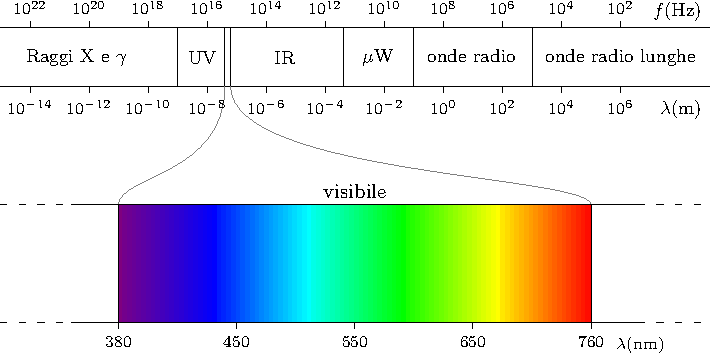
\includegraphics[width=0.8\textwidth]{spettroelettromagnetico}
    \caption{Composizione dello spettro delle onde elettromagnetiche}
    \label{fig:spettroelettromagnetico}
  \end{figure}
\clearpage




\section{Classificazione di immagini telerilevate}

\subsection{Premessa}

Si definisce classificazione di immagini telerilevate, il processo di assegnazione di una "etichetta" a ciascun pixel dell'immagine, in modo tale da renderlo appartenente ad una specifica classe, raprresentativa di una data copertura di suolo.
La classificazione è il primo step del processo di estrapolazione di dati di carattere informativo da una immagine telerilevata, che vengono forniti, poi, alle successive fasi di riconoscimento (\emph{matching}) ed interpretazione. 
Queste tre fasi compongono la disciplina del \emph{Pattern Recognition}, il cui obiettivo è appunto sviluppare tecniche con cui implementare i tre processi.
Oltre alla generazione di mappe tematiche tramite sistemi di telerilevamento, il \emph{pattern recognition} abbraccia vari ambiti quali l'analisi di immagini biomedicali, orientate alla robotica (\emph{Computer Vision}), o per la videosorveglianza.   

%-----------------------------------
%	SUBSECTION 2
%-----------------------------------

\subsection{Spazi di rappresentazione}

Esistono tre principali metodologie di rappresentazione dei dati, la rappresentazione nello "spazio-immagine" (\emph{Image Space}), la rappresentazione nello "spazio spettrale" (\emph{Spectral Space}) e quella nello "spazio delle features" (\emph{Fautures Space}). La prima e più immediata consiste nel visualizzare i dati canale per canale tramite terne RGB, in modo tale che ogni banda risulti una immagine a sé. La seconda tipologia consiste, invece, nel visualizzare per ciascun pixel, i livelli di grigio di ogni canale, per rappresentarli poi in un grafico. La rappresentazione nello "spazio delle \emph{feature}" si basa sull'assegnazione di assi cartesiani distinti ad ogni banda, e, così facendo, ad ogni pixel viene assopciato un vettore n-dimensionale, con n il numero di canali. Quest'ultima rappresentazione non solamente evidenzia i livelli di grigio dei pixel ma anche la distribuzione statistica nelle varie bande, rendendola generalmente piu vantaggiosa rispetto alle altre due in quanto a differenti distribuzioni nello spazio delle feature corrispondono tipicamente a differenti coperture di suolo.  

\begin{figure}[!ht]
\center
\subfigure[Rappresentazione nello spazio spettrale di un pixel di una immagine iperspettrale (220 canali) ottenuta tramite AVIRIS.]{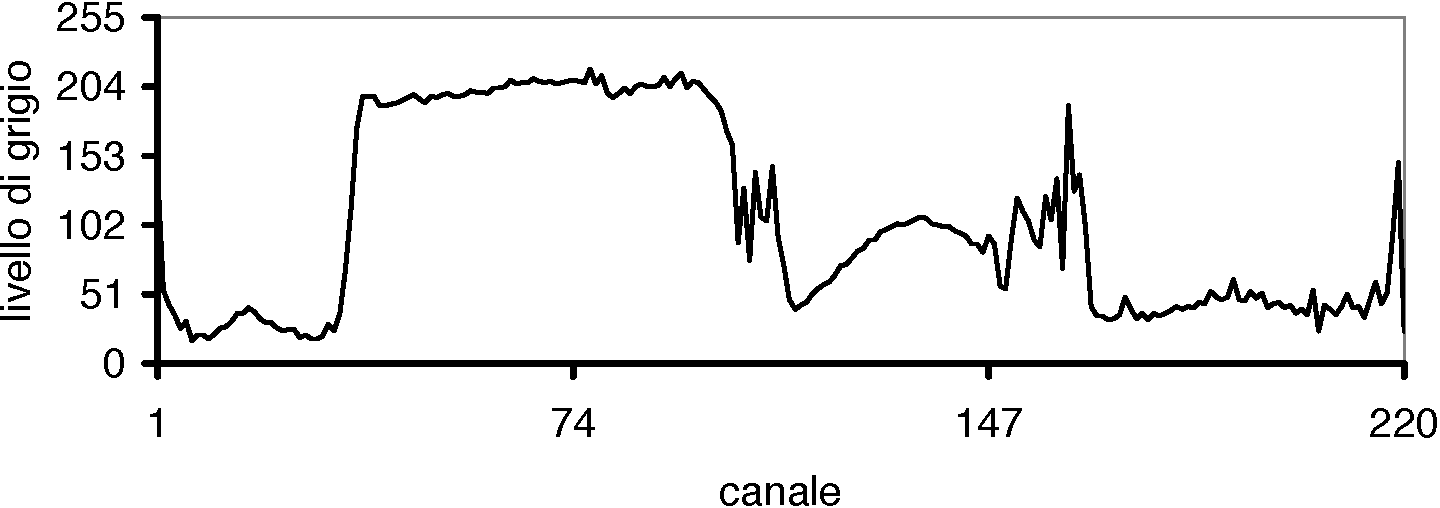
\includegraphics[width=0.4\textwidth]{indianpine_spectral}}
\hspace{3mm}
\subfigure[Rappresentazione nello spazio immagine.]{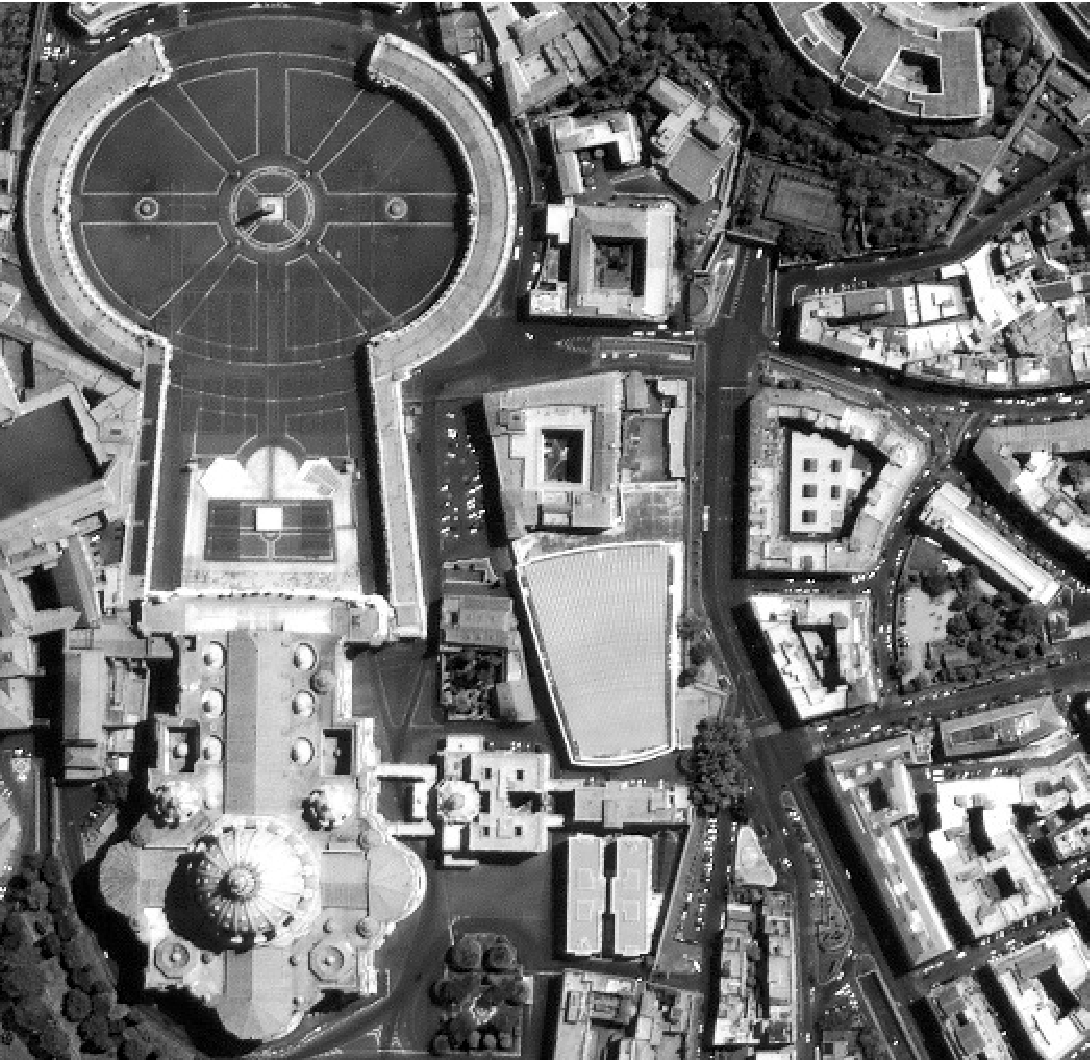
\includegraphics[width=0.4\textwidth]{vaticano}}
\\
\subfigure[Rappresentazione nello spazio delle feature.]{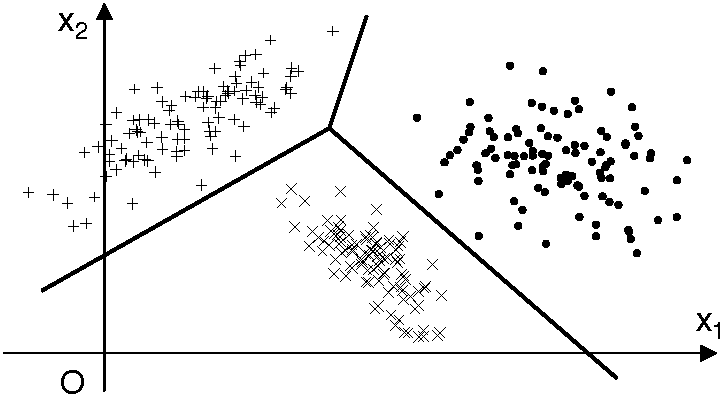
\includegraphics[width=0.5\textwidth]{featurespace}}
\caption{Esempi di rappresentazione in diversi spazi.}
\label{fig:spaziorappresentazione}
\end{figure}



%-----------------------------------
%	SUBSECTION 3
%-----------------------------------
\subsection{La classificazione nello spazio delle \emph{feature}}

A fini di classificazione, la rappresentazione nello spazio delle \emph{feature} si rivela, solitamente, la più vantaggiosa, in quanto gli andamenti spettrali di pixel appartenenti a classi distinte possono essere maggiormente separabili. In quest'ottica, classificare significa quindi partizionare lo spazio delle "feature" in opportuni sottoinsiemi, ciascuno associato ad una data classe.
\\

I classificatori possono essere divisi in due macro-famiglie, classificatori supervisionati (\emph{supervised}) e non supervisionati (\emph{unsupervised}). La prima tipologia prevede principalmente due fasi, una fase iniziale di addestramento (\emph{training}) e una di verifica (\emph{test}); nel primo step, il sistema ottimizza parametri del classificatore tramite un insieme di pixel preclassificati (\emph{training} set), fino a raggiungere una adeguata accuratezza. Successivamente, il sistema viene testato in modo analogo alla fase di training, attraverso un insieme di pixel preclassificati ma differenti rispetto a quelli coinvolti nella fase di \emph{training}.\\
Nei classificatori non supervisionati, invece, non viene utilizzato alcun \emph{training set}, solitamente perchè non sono note nè facilmente identificabili le classi coinvolte nell'applicazione in esame. 
\\

Nei capitoli a seguire la nostra attenzione sarà focalizzata sul concetto di classificazione supervisionata, che si basa, in generale, su tre assunti:
\begin{itemize}
\item si ha una conoscenza a priori esaustiva su un sottoinsieme di pixel preclassificati (\emph{training set});
\item le classi esistono in numero finito e sono note \emph{ex ante};    
\item ogni pixel è rappresentabile tramite un insieme di valori detti vettore delle \emph{feature} (\emph{feature vector}).
\end{itemize}


\subsubsection*{Concetti chiave e definizioni}
Data un immagine telerilevata, a ciascun pixel $(m,n) \in \mathbb{Z}$ può essere associato un vettore d-dimensionale delle \emph{feature} $\textbf{x}(m,n)\in \mathbb{R}^d$, le cui componenti (le d \emph{feature}) possono essere non solamente i livelli di grigio dei pixel $(m,n)$ nelle varie bande, ma anche parametri aggiuntivi come ad esempio i cosiddetti parametri di tessitura (o \emph{feature} di tessitura).\\

Le \emph{feature} di tessitura vengono estratte al fine di analizzare le differenze nella distribuzione spaziale dei livelli di grigio dei pixel, permettendo di distinguere coperture di suolo differenti. In generale, se i pixel estratti da classi differenti sono situati in zone disgiunte dello spazio delle feature, la accuratezza di classificazione è tanto maggiore quanto più sono separate le regioni. Se infatti, in una stessa regione si trovano classi distinte, esse risulteranno sovrapposte e quindi distinguerle risulterà largamente più difficoltoso.
\\

Dato un insieme $\Omega =\lbrace\omega_1,\ldots, \omega_c\rbrace$ costituito da $C$ classi distinte, note a priori, si assume che ogni oggetto o entità da analizzare sia appartenente ad una ed una sola classe (nel nostro caso ad una data copertura del suolo). A ciascun pixel è associata, quindi, anche un'etichetta di classe $y(m,n) \in \Omega$ e l'immagine $y(m,n)$ (con $m,n\in \mathbb{Z}$) è detta mappa di classificazione.
\\

Il \emph{training set} è l'insieme dei pixel di cui è nota a priori l'etichetta di classe ed è definito dall'insieme delle coppie $\left\lbrace \mathbf{x}_i,y_i \right\rbrace $, $i=1,\ldots,N$ con $N$ il numero di vettori di \emph{training} scelti. L'insieme di tali etichette rappresenta un'ulteriore immagine, detta  \emph{mappa di training}, che evidenzia alcuni pixel dell'immagine assegnati a ciascuna classe, distinguendoli dai "pixel di sfondo", cioè quei pixel per i quali l'etichetta di classe è incognita.
\\
Il processo di classificazione, come già accennato precedentemente, è diviso in due passi: \emph{learning} e \emph{prediction} (fase di addestramento e fase di predizione). Lo scopo della fase di \emph{learning} è quello di costruire un modello di classificatore, tramite la definizione di una \emph{regola di decisione} (o anche detta \emph{funzione discriminante}). \\
In termini generali, la \emph{regola di decisione} è una funzione $f:\mathbb{R}^d\rightarrow\mathbb{R}$ modellata sulla base dell'andamento statistico del \emph{training set} in modo tale che $f$ valutata per un pixel incognito restituisca una stima dell'etichetta da associarci. Le funzioni discriminanti possono essere definite con vari metodi, cui corrispondono varie tecniche di classificazione (nel Capitolo \ref{cap:svm} ne viene descritto uno dei possibili). \\
Conclusa questa fase, si procede con la classificazione vera e propria: si scansiona l'intera immagine valutando ogni pixel tramite la \emph{regola di decisione}, realizzando, in questo modo, una stima della mappa di classificazione.

\tikzstyle{block} = [rectangle, draw, %fill=blue!20, 
     text width=8em, text centered, rounded corners, minimum height=3em]
\tikzstyle{arrow} = [draw, -latex]
\tikzstyle{line} = [draw]


\begin{figure}[!ht]
\center
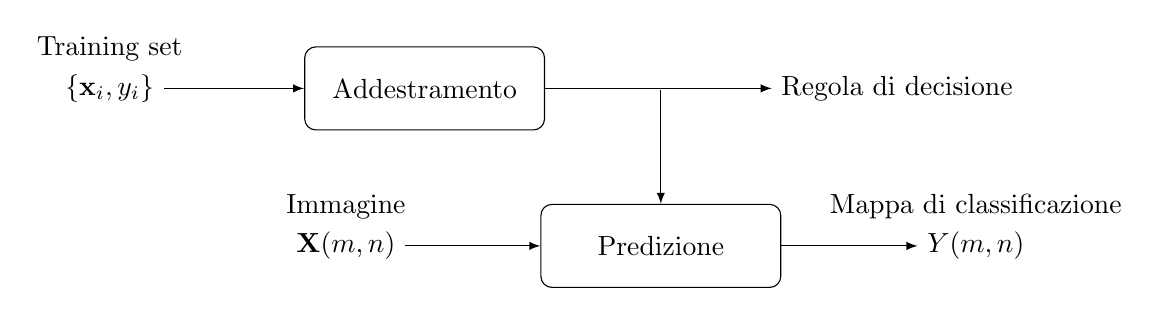
\begin{tikzpicture}
\node[](training) at (0,0) {$\left\lbrace \mathbf{x}_i,y_i \right\rbrace $};
\node[] at (0,.5){Training set};
\node[block] (addestramento) at (4,0) {Addestramento};
\node[](decision_rule) at (10,0) {Regola di decisione};
\node[](node1) at (7,.1){};
\node[block](prediction) at (7,-2) {Predizione};

\node[](image) at (3,-2) {$ \mathbf{X}(m,n)$};
\node[] at (3,-1.5){Immagine};

\node[]() at (11,-1.5) {Mappa di classificazione};
\node[](classmap) at (11,-2) {$Y(m,n)$};

\path[arrow] (training)--(addestramento);
\path[arrow] (addestramento) -- (decision_rule);
\path[arrow] (node1)--(prediction);
\path[arrow] (image)--(prediction);
\path[arrow] (prediction)--(classmap);
\end{tikzpicture}
    \caption{Schema funzionale di un classificatore}
    \label{fig:flowchart_classificatore}
  \end{figure}
\clearpage


\section{Il ruolo dell'informazione spaziale}

Una ulteriore distinzione che permette di differenziare tra loro le tipologie di classificatori è quella inerente al ruolo dei pixel adiacenti nella analisi della copertura al suolo. Esistono, infatti, classificatori cosiddetti non contestuali, in cui la copertura viene analizzata senza tener conto dei pixel adiacenti, risparmiando così un alto costo computazionale, ma trascurando la forte correlazione tra pixel limitrofi. Infatti, la probabilità che una zona sia formata da pixel tutti appartenenti alla stessa classe è molto elevata; si pensi solamente a zone boschive o fluviali in cui tali regioni possono estendersi per chilometri. 
\\

Queste due tipologie di classificatori sono chiaramente differenti anche in base all'ambito in cui vengono applicate; mentre le tecniche di classificazione supervisionata non contestuale risultano molto efficaci e largamente consolidate per le immagini con una risoluzione piuttosto grossolana, mostrano forti limiti per le immagini \emph{Very High Resolution}. 
Una maggiore risoluzione spaziale comporta, infatti, una maggiore eterogeneità e una corrispondente buona definizione delle strutture geometriche quali strade e edifici, caratteristiche che rendono necessario l'utilizzo di classificatori contestuali. 
A tal fin, un ruolo chiave viene giocato principalmente da tre approcci metodologici, l'estrazione di parametri di tessitura, metodi basati su regioni e oggetti e i \emph{Markov Random Fields} (MRF).


\subsection{Estrazione dei parametri di tessitura}
L'estrazione di \emph{texture} ha come obiettivo quello di rilevare, in una determinata regione dell'immagine, strutture ripetitive nella distribuzione spaziale dei pixel quali zone urbane o boschive. 
Ciò fornisce una sorgente di dati complementare per le applicazioni in cui l'informazione relativa unicamente allo spettro dell'immagine risulta non sufficiente ai fini della classificazione. 
Le principali tecniche di estrazione di parametri di tessitura si basano sui semivariogrammi, che consistono in una statistica del secondo ordine delle intensità dei pixel, sulla morfologia matematica o addirittura su metodi che coinvolgono finestre mobili in cui vengono effettuate analisi non sul singolo pixel ma su una intera zona adiacente. 


\subsection{Tecniche Region-based}
Gli approcci basati invece sulle regioni (\emph{region-based methods}) si basano su tecniche che puntano a suddividere le immagini in segmenti o regioni omogenee. In generale, una buona tecnica di segmentazione possiede:
\begin{itemize}
\item pixel nella stessa categoria aventi livelli di grigio simili e formano una regione connessa;
\item pixel adiacenti che sono in categorie differenti hanno valori differenti. 
\end{itemize}


\subsection{Markov Random Fields}
I \emph{Markov Random Fields}, che generalizzano il concetto di catena markoviana monodimensionale ad un sistema 2D, massimizzano l'accuratezza tramite la dipendenza che sussiste tra pixel adiacenti. 
Esso offre, infatti, una soluzione computazionalmente efficiente per restringere la zona di interesse dall'intera immagine (elaborazione globale) ad un intorno del pixel (elaborazione locale). 
In particolare, siano $i$ e $j$ due pixel dell'immagine, si ha allora che se la funzione di probabilità $P(Y)>0$ per ogni configurazione $Y$ e se la seguente condizione è garantita per tutti i pixel i dell'immagine:
\begin{equation}
P(y_i|y_j, j \neq i) = P(y_i|y_j, j\sim i)
\end{equation}   
Ciò indica che la distribuzione di probabilità delle etichette di ciascun pixel $i$, condizionata ai valori di tutti gli altri pixel dell'immagine, può essere ristretta alla distribuzione delle etichette di $i$ condizionato solamente alle etichette dei pixel adiacenti. Si può chiaramente osservare come tale definizione sia una generalizzazione dei processi markoviani monodimensionali, in cui la probabilità di transizione da uno stato ad un altro dipende unicamente dallo stato precedente.
    

